\documentclass{article}
\usepackage[utf8x]{inputenc}
\usepackage{ucs}
\usepackage{amsmath} 
\usepackage{mathtext}
\usepackage{amsfonts}
\usepackage{marvosym}
\usepackage{wasysym}
\usepackage{upgreek}
\usepackage[english,russian]{babel}
\usepackage{graphicx}
\usepackage{float}
\usepackage{textcomp}
\usepackage{hyperref}
\usepackage{geometry}
  \geometry{left=2cm}
  \geometry{right=1.5cm}
  \geometry{top=1cm}
  \geometry{bottom=2cm}
\usepackage{tikz}
\usepackage{ccaption}
\usepackage{multicol}
\usepackage{hyperref}



\usepackage{listings}
%\setlength{\columnsep}{1.5cm}
%\setlength{\columnseprule}{0.2pt}

\usepackage[absolute]{textpos}

\begin{document}
\pagenumbering{gobble}

\lstset{
  language=C,                % choose the language of the code
  basicstyle=\linespread{1.1}\ttfamily,
  columns=fixed,
  fontadjust=true,
  basewidth=0.5em,
  keywordstyle=\color{blue}\bfseries,
  commentstyle=\color{gray},
  stringstyle=\ttfamily\color{orange!50!black},
  showstringspaces=false,
  %numbers=false,                   % where to put the line-numbers
  numbersep=5pt,
  numberstyle=\tiny\color{black},
  numberfirstline=true,
  stepnumber=1,                   % the step between two line-numbers.        
  numbersep=10pt,                  % how far the line-numbers are from the code
  backgroundcolor=\color{white},  % choose the background color. You must add \usepackage{color}
  showstringspaces=false,         % underline spaces within strings
  captionpos=b,                   % sets the caption-position to bottom
  breaklines=true,                % sets automatic line breaking
  breakatwhitespace=true,         % sets if automatic breaks should only happen at whitespace
  xleftmargin=.2in,
  extendedchars=\true,
  keepspaces = true,
}
\lstset{literate=%
   *{0}{{{\color{red!20!violet}0}}}1
    {1}{{{\color{red!20!violet}1}}}1
    {2}{{{\color{red!20!violet}2}}}1
    {3}{{{\color{red!20!violet}3}}}1
    {4}{{{\color{red!20!violet}4}}}1
    {5}{{{\color{red!20!violet}5}}}1
    {6}{{{\color{red!20!violet}6}}}1
    {7}{{{\color{red!20!violet}7}}}1
    {8}{{{\color{red!20!violet}8}}}1
    {9}{{{\color{red!20!violet}9}}}1
}

\begin{textblock*}{5cm}(14cm,2cm)
  \raggedright
  \textbf{\Circpipe} -- вопрос \\
  \textbf{\Squarepipe} -- задача \\
  \textbf{\Bat} -- продвинутая задача
\end{textblock*}

\section*{\hfil Задание для подготовки к Контрольной работе \#2 \hfil}

\section*{Указатели}

\subsection*{Основы работы с указателями}

\subsubsection*{Адреса переменных. Операция получения адреса}
Каждая переменная в языке C хранится где-то в памяти и имеет адрес. Адрес переменной это просто номер первого байта соответствующей области памяти.  Чтобы получить адрес переменной нужно перед переменной поставить \&(амперсанд). Обычно адреса записываются в шестнадцатеричной системе счисления, например 0x7FFFB014 это адрес ячейки под номером 2147463188 (такое число получится если перевести 0x7FFFB014 из шестнадцатеричной системы в десятичную).
\begin{lstlisting}
double x = 123.456;
printf("Address of x is: %p\n", &x);
\end{lstlisting}

\subsubsection*{Объявление указателей}
Указатель это переменная, которая хранит адреса переменных. Тип указателя такой: <тип переменной>*. Тип переменной, на которую указывает указатель, нужно знать, чтобы правильно выполнять операцию разыменования. Если тип переменной, на которую будет указывать указатель, не известен, то можно использовать указатель \texttt{void*}. Размер указателя обычно равен 4 байта на 32-х битных системах и 8 байт на 64-х битных. Так как указатель это переменная, то у него тоже есть адрес. Пример:
\begin{lstlisting}
int a = 100;  // Переменная типа int, присвоено значение, равное 100
int* q;       // Переменная типа указатель на int, значение не присвоено
int* p = &a;  // Переменная типа указатель на int, присвоено значение, равное адресу a
void* pv = &a;// Переменная типа ' указатель на что - то ', присвоено значение, равное адресу a
\end{lstlisting}

\subsubsection*{Операция разыменования}
Чтобы доступиться к переменной по указателю нужно поставить символ * перед указателем. Операция получения значения переменной по указателю называется операцией разыменования.
\begin{lstlisting}
int a = 100;
int* p = &a; // Теперь можно использовать a с помощью p. Можно сказать, что *p это синоним a.
printf("%d", *p);   // Напечатает 100
*p += 10;           // Значение переменной a увеличится на 10
void* pv = &a;
printf("%d", *pv); // Неправильно, так как неизвестно какой тип у *pv.
\end{lstlisting}

\subsubsection*{Арифметика указателей. Операции, которые можно производить с указателями:}
\begin{enumerate}
\item Присваивание другому указателю или адресу.
\begin{lstlisting}
float a[5] = {1.2, 3.4, 5.6, 7.8, 9.0};
float* p = &a[3];
char* pc = &a[0];  // Warning: Слева и справа разные типы. Тем не менее в языке C это не ошибка и работать будет. Указатель float* приведётся к указателю char*.
\end{lstlisting}
\item Сравнение двух указателей. Операция \texttt{==}
\item Сложение указателя с целым числом. Возвращается указатель, смещённый на n * sizeof(type)
\begin{lstlisting}
p = p + 3; // p увеличится 3 * sizeof(float)
\end{lstlisting}
\item Вычитание двух указателей. Возвращается разница двух адресов, делённая на sizeof(type).
\begin{lstlisting}
printf("%lu", p - a); // Напечатает 3. Массив часто ведёт себя как указатель на 0 элемент 
\end{lstlisting}
\item Операция взятия индекса: \texttt{p[2], p[-1], a[3]} и т. д. \\
\textbf{\texttt{a[i]} это то же самое что и \texttt{*(a + i)}.}
\end{enumerate}

\subsubsection*{\Squarepipe \quad Задача \#1: Адрес}
Пусть есть указатель p на переменную типа int, которая имеет адрес 0x7FFFB014. Переменная int на рассматриваемой системе имеет размер 4. Чему равны значения (в шестнадцатеричной системе счисления):
\begin{multicols}{3}
\begin{itemize}
\item p + 1
\item p + 2
\item p + 6
\end{itemize}
\end{multicols}

\subsection*{Применение указателей}
\subsubsection*{Передача адресов переменных в функцию}
Указатели часто используются чтобы изменять передаваемые значения в функциях:
\begin{multicols}{2}
\begin{lstlisting}
// Неправильно:
void normalize(float x, float y)
{
    float sum = x + y;
    x = x / sum;
    y = y / sum; 
    // Изменятся x и y - копии a и b
}
// ...
float a = 20.0, b = 80.0;
normalize(a, b);
// a и b не изменятся: a=20.0, b=80.0
\end{lstlisting}
\begin{lstlisting}
// Правильно:
void normalize(float* x, float* y)
{
    float sum = *x + *y;
    *x = *x / sum;
    *y = *y / sum; 
    // Изменятся переменные a и b
}
// ...
float a = 20.0, b = 80.0;
normalize(&a, &b);
// a и b изменятся:a=0.2, b=0.8
\end{lstlisting}
\end{multicols}

\subsubsection*{\Squarepipe \quad Задача \#2: Передача по адресу}
Написать функцию \texttt{void make\_positive(float* x)}, которая делает число положительным. Например:
\begin{lstlisting}
float x = -1.2; y = 4.5;
make_positive(&x); // x изменится и станет равным 1.2
make_positive(&y); // y не изменится
\end{lstlisting}

\subsubsection*{Передача в функцию с использованием указателя на константу}
Ещё один часто используемый способ передачи в функцию -- передача с использованием указателя на константу
\begin{lstlisting}
void some_func(const float* p)
{
	printf("%f\n", *p);  // ОК
	*p = 10.0;           // Неправильно! 
	// Нельзя менять то, на что указывает p, так как используется const
}
\end{lstlisting}

\textbf{\Circpipe} Какие преимущества такой передачи по сравнению с обычной передачей и передачей с использованием указателя? Когда следует использовать такой способ передачи?
\newpage

\section*{Структуры}
\setlength{\columnsep}{1.5cm}
\setlength{\columnseprule}{0.2pt}
\begin{multicols}{2}
\subsubsection*{Объявление структуры}
\begin{lstlisting}
struct city
{
    char name[50];   // Название города
    int population;  // Население
    float area;      // Площадь города
};
typedef struct city City;   
\end{lstlisting}

\subsubsection*{Создание экземпляра структуры}
\begin{lstlisting}
City x = {"Moscow", 12228685, 2511.0};
x.area *= 2; // Увеличим площадь в 2 раза
City best_cities[] = {
    {"New York", 8175133, 1213.37},
    {"Tokyo", 13617445, 2187.66 },
    {"Shanghai", 24152700, 6341.0},
    {"Dolgoprudniy", 104238, 30.52}};
\end{lstlisting}
\subsubsection*{Передача структуры в функцию}
Структуры в функции передаются как обычные переменные
\begin{lstlisting}
// Передача по значению (x копируется)
void print_name(City x)
{
    printf("%s", x.name);
    // Используем точку .
}
// Передача через указатель
void increase_population(City* p, int n)
{
    p->population += n;
    // Используем стрелочку ->
}
\end{lstlisting}
\end{multicols}
Рассмотрим задачу парсирования из строки в структуру. Предположим, что информация о городе записана в строке в следующем формате: \texttt{char str[100] = ``Moscow-12228685-2511.0''}, тогда для считывания из строки и записи нужных значений в структуру можно использовать функцию \texttt{sscanf()}: 
\begin{lstlisting}
char str[100] = ``Moscow-12228685-2511.0'';
City a;
sscanf(str, "%[^-]-%d-%f, , &a.name, &a.population, &a.area");
// Выражение %[^-] означает считываем всё до знака - в строку
\end{lstlisting}

\subsubsection*{\Squarepipe \quad Задача \#3: Парсим координаты}
\begin{itemize}
\item Объявите структуру Point, описывающую точку в пространстве. Эта структура должна иметь поля x, y, z типа float. 
\item Напишите функцию \texttt{void print\_point(Point a)}, которая принимает на вход эту структуру и печатает её на экран в следующем формате: (x, y, z).
\item Предположим, что информация о точке записана в строке в следующем формате: \texttt{char str[50] = ``(1.5, 4.0, 3.7)''}. Создать новую структуру Point и считать информацию из строки в эту структуру с помощью sscanf().
\item Напишите функцию \texttt{Point parse\_point(char* str)}, которая считывает информацию из строки \texttt{str} в структуру и возвращает эту структуру. Нужно использовать функцию \texttt{sscanf()}.
\end{itemize}
Следующий код должен выводить на экран координаты, записанные в строках s1 и s2:
\begin{lstlisting}
int main()
{
    char s1[] = "(3.2, 535.0, -74.78)";
    char s2[] = "(-777, 0.000, 123456789.987654321)";
    Point a = parse_point(s1);
    Point b = parse_point(s2);
    print_point(a);
    print_point(b);
}
\end{lstlisting}
\newpage
\section*{Строки}
\subsubsection*{Символы}
\begin{multicols}{2}
Тип char -- тип целых чисел от -128 до 127\\
Символы кодируются в соответствии с таблицей ASCII,
например, символ '9' это просто число 57.
\begin{lstlisting}
char a = 100; // Как число от -128 до 127
char b = 'A'; // Как символ
if ('9' == 57)
    printf("Char is a number\n");
\end{lstlisting}
Некоторые символы ASCII:\\
\begin{tabular}{ c | c | c }
  {\color{red}\textbf{'0'}} = 48 & {\color{red}\textbf{'A'}} = 65 & нулевой символ  {\color{red}\textbf{'\textbackslash 0'}} = 0 \\
  {\color{red}\textbf{'1'}} = 49 & {\color{red}\textbf{'B'}} = 66 & символ переноса строки {\color{red}\textbf{'\textbackslash n'}} = 10 \\
  {\color{red}\textbf{'2'}} = 50 & ...                             & табуляция {\color{red}\textbf{'\textbackslash t'}} = 9 \\
  ...                            & {\color{red}\textbf{'Z'}} = 90 & backspace {\color{red}\textbf{'\textbackslash b'}} = 8 \\
  {\color{red}\textbf{'9'}} = 57 & {\color{red}\textbf{'a'}} = 97 & звуковой сигнал {\color{red}\textbf{'\textbackslash a'}} = 7 \\
  {\color{red}\textbf{' '}} = 32 & ...                           & возврат каретки {\color{red}\textbf{'\textbackslash r'}} = 13 \\
                                 & {\color{red}\textbf{'z'}} = 122  &   \\
\end{tabular}
\end{multicols}

\subsubsection*{Строки как массив символов}
Строка это просто массив из символов. Строка должна заканчиваться символом '\textbackslash 0'.
\begin{lstlisting}
char s1[10];          // Объявление строки
char s2[10] = "abc";  // Объявление + инициализация

s1 = "xyz"; // Неправильно! Так присваивать строки нельзя, так как строка это просто массив
strcpy(s1, "xyz"); // Чтобы присвоить строке значение нужно использовать функцию strcpy()
                   // Для использования функций работы со строками нужно подключить <string.h>
\end{lstlisting}

\subsubsection*{\Squarepipe \quad Задача \#4: Обращение строки}
Написать функцию \texttt{void reverse(char* str)}, которая переворачивает строку.

\subsubsection*{\Squarepipe \quad Задача \#5: Шифр Цезаря}
Написать функцию \texttt{void encrypt(char* str)}, которая изменяет строку следующим образом: все символы 'a' меняются на 'b', все символы 'b' меняются на 'c' ... все символы 'z' меняются на 'a'. То же самое для заглавных букв. Остальные символы не меняются.

\subsubsection*{Функции для работы со строками}
\begin{itemize}
\item \texttt{strlen(str)} -- вычисляет количество символов в строке str.
\item \texttt{strcpy(dest, src)} -- копирует содержимое строки src в строку dest.
\item \texttt{strcmp(str1, str2)} -- сравнивает строки str1 и str2. Возвращает 0, если они равны.
\item \texttt{strstr(str, substr)} --  возвращает указатель на первый символ вхождения строки substr в строку str.
\item \texttt{strcat(str1, str2)} -- добавляет строку str2 в конец строки str1.
\end{itemize}
\subsubsection*{\Squarepipe \quad Задача \#6: Строка + указатели} Предположим, что задана строка \texttt{char str[100] = ``A bicycle can't stand on its own because it is two-tired''}, что напечатают следующие строки:
\begin{multicols}{2}
\begin{itemize}
\item \texttt{printf(``\%lu'', strlen(str))}
\item \texttt{printf(``\%s'', str)}
\item \texttt{printf(``\%s'', str + 33)}
\item \texttt{printf(``\%s'', strstr(str, ``bec''))}
\item \texttt{printf(``\%lu'', strstr(str, ``can'') - str)}
\end{itemize}
\end{multicols}

\newpage

\section*{Динамическое выделение памяти}
\begin{lstlisting}
int* arr = malloc(n * sizeof(int));
// ...  
free(arr);
\end{lstlisting}
\subsubsection*{\Squarepipe \quad Задача \#7: Среднее и дисперсия + malloc()}
На вход программе подаётся целое число $n$ и $n$ вещественных чисел типа double ${x_i}$. Нужно найти среднее этих чисел $\mu$ и дисперсию $D$. Для выделения памяти используйте malloc() и free(). 
\begin{align*}
  \mu = \frac{1}{n}\sum_{i=0}^{n-1}x_i & \quad \quad \quad \quad D = \frac{1}{n}\sum_{i=0}^{n-1}(x_i - \mu)^2
\end{align*}

\subsubsection*{Выделение памяти для 2D массива}
Сначала нужно выделить память для указателей на строки. А затем выделить память для каждой из строк.
\begin{lstlisting}
// Выделяем память под 2D массив
int** A = malloc(n * sizeof(int*));
for (int i = 0; i < n; ++i)
	A[i] = malloc(m * sizeof(int));
// Работаем с 2D массивом A как с обычным 2D массивом
// ...  
// Освобождаем память
for (int i = 0; i < n; ++i)
	free(A[i]);
free(A);
\end{lstlisting}

\subsubsection*{\Squarepipe \quad Задача \#8: Malloc 2D}
На вход программе подаются 2 целых числа n и m. Затем на вход подаются $n \times m$ вещественных чисел типа. Нужно напечатать матрицу, отзеркаленную по вертикали. Всю необходимую память выделить динамически.
\section*{Сортировка (qsort)}
\begin{multicols}{2}
Сортировка чисел:
\begin{lstlisting}
int cmp_int(const void* a, const void* b)
{
    int* pa = (int*)a;
    int* pb = (int*)b;
    return (*pa - *pb);
}



int main ()
{
    int arr[] = {8, 2, 5, 1};
    qsort(arr, 4, sizeof(int), cmp_int);
}
\end{lstlisting}
Сортировка структур:
\begin{lstlisting}
int cmp_city(const void* a, const void* b)
{
    City* pa = (City*)a;
    City* pb = (City*)b;
    return (pa->population -
            pb->population);
}
int main ()
{
    City arr[] = {{``A'', 78, 5.4}, 
                  {``B'', 54, 1.9}, 
                  {``C'', 97, 4.2}};
    qsort(arr, 3, sizeof(City), cmp_city);
}
\end{lstlisting}
\end{multicols}
\subsubsection*{\Squarepipe \quad Задача \#9: Сортировка}
Создать массив структур City и инициализировать его 5-ю различными городами. Отсортировать этот массив по плотности населения.
\section*{Файлы}
\begin{multicols}{2}
Считывание/запись.
\begin{lstlisting}
FILE* fin = fopen("input.txt", "r");
int x, y, z;
fscanf(fin,"%d%d%d", &x, &y, &z);
fclose(fin);


FILE* fout = fopen("output.txt", "w");
fprintf(fout,"Hello file!\n");
fclose(fout);
\end{lstlisting}
Посимвольное считывание/запись.
\begin{lstlisting}
FILE * f = fopen("input.txt", "r");
int c, number_of_digits = 0;

while ((c = fgetc(f)) != EOF)
{
    if (c >= '0' && c <= '9')
        number_of_digits += 1;
}
fclose(f);
\end{lstlisting}
\end{multicols}
\subsubsection*{\Squarepipe \quad Задача \#10: Среднее и дисперсия + malloc() + file}
Решить задачу \#7, но только считывание должно проводится не из стандартного входа, а из файла ``input.txt''.
\subsubsection*{\Squarepipe \quad Задача \#11: Количество слов в файле.}
Посчитать число слов в файле ``input.txt''. Слово это любая последовательность символов, разделённая пробелом, символом табуляции('\textbackslash t') или символом перевода строки('\textbackslash n').

\subsubsection*{\Bat \quad Задача \#12: qraces}
Решить задачу qraces-1 из контрольной работы 2015-2016 + добавить считывание из файла ``input.txt'' и запись в файл ``output.txt''.

\section*{Связный список}
\begin{center}
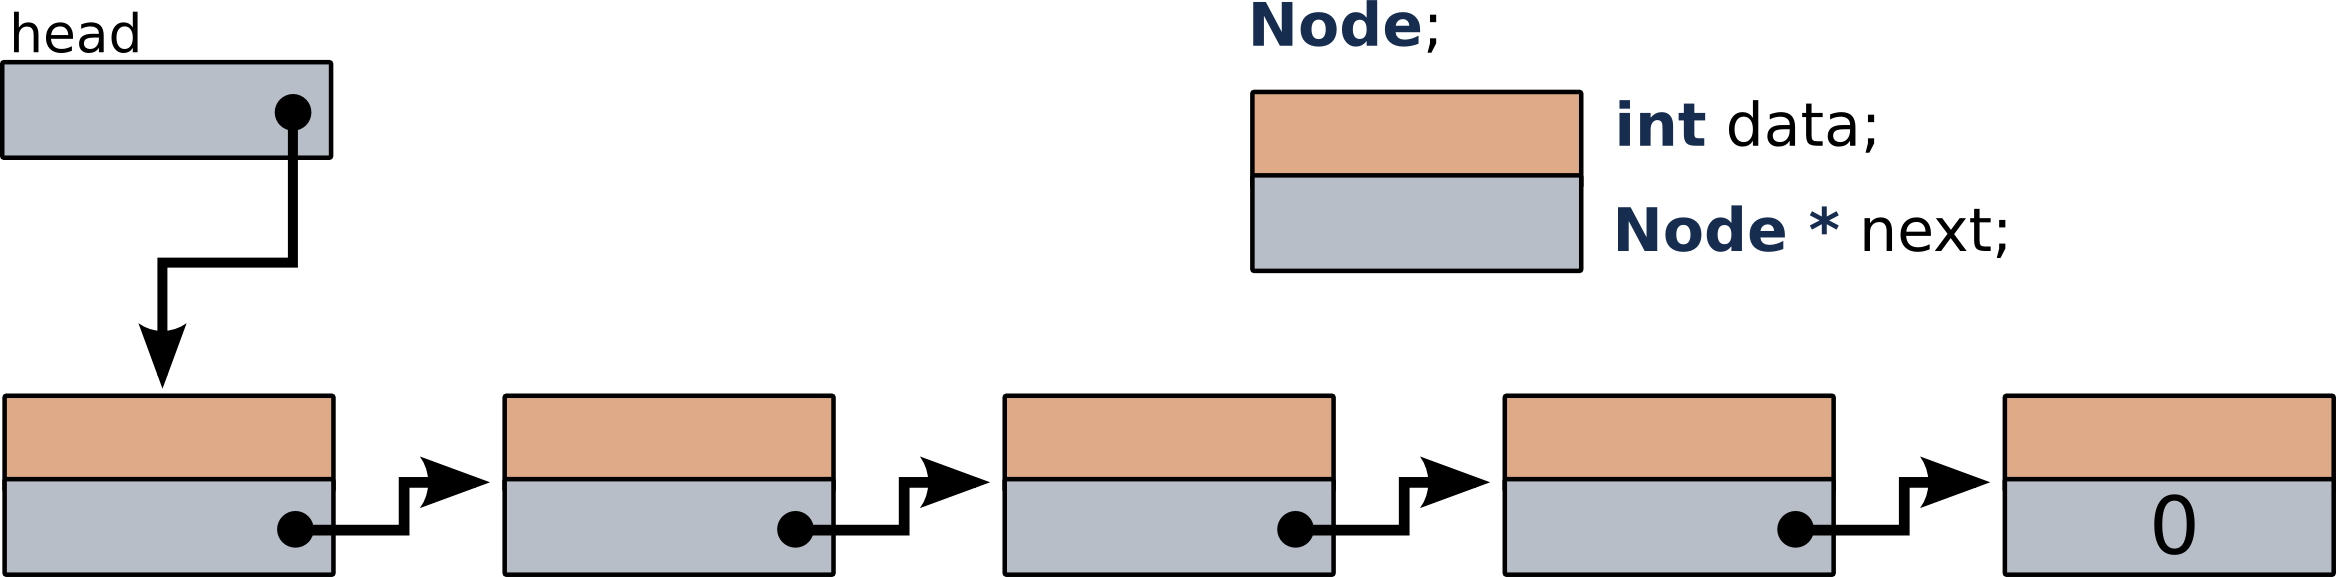
\includegraphics[width=0.6\linewidth]{list_initial.png}\\
\end{center}
Базовый исходный код связного списка можно найти тут:\\
\href{https://github.com/v-biryukov/cs_mipt_faki/tree/master/term1/seminar11_list/programms}{github.com/v-biryukov/cs\_mipt\_faki/tree/master/term1/seminar11\_list/programms}

\subsubsection*{\Squarepipe \quad Задача \#13 Перевернуть список}
Написать функцию \texttt{void list\_reverse(Node** p\_head)}, которая переворачивает связный список. Первый элемент становится последним, а последний первым. 

\subsubsection*{\Bat \quad Задача \#14 Есть ли цикл}
Написать функцию \texttt{int list\_is\_loop(Node* head)}, которая проверяет, если в связном списке цикл.

\subsubsection*{\Bat \quad Задача \#15 Устранить цикл}
Написать функцию \texttt{int list\_is\_loop(Node** p\_head)}, которая проверяет, если в связном списке цикл и если цикл есть, то он устраняется. Подробней можно прочитать тут:

\href{http://www.geeksforgeeks.org/detect-and-remove-loop-in-a-linked-list/}{www.geeksforgeeks.org/detect-and-remove-loop-in-a-linked-list}


\end{document}